




\begin{figure*}[t]

\centerline{
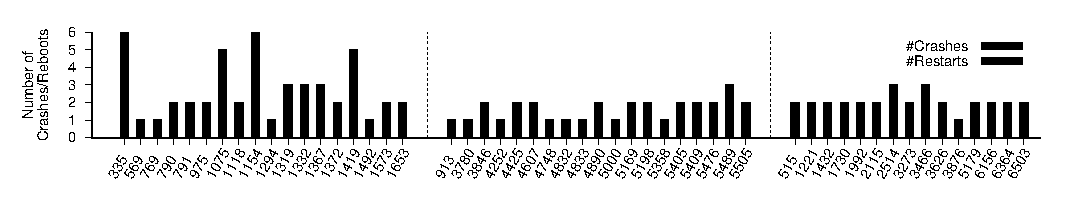
\includegraphics[width=6.5in]{F/deepbugs/eps/all.eps}
%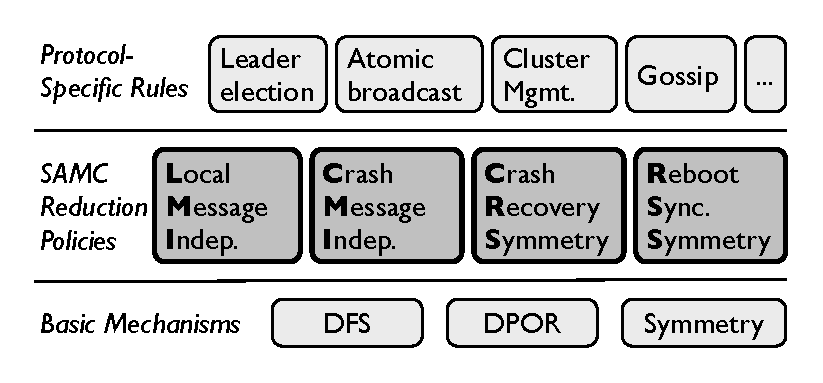
\includegraphics[height=1.2in]{F/samc/samc.eps}
}
\scriptsize{
~~~~~~~~~~~~~~~~~~~~~~~~~~~~~~~~~~~~~~\textsf{ZooKeeper Bugs}
~~~~~~~~~~~~~~~~~~~~~~~~~~~~~~~~~~~~\textsf{Hadoop MapReduce Bugs}
~~~~~~~~~~~~~~~~~~~~~~~~~~~~~~~\textsf{Cassandra Bugs}}
\vminfive
\mycaption[Deep Bugs]{fig-deepbugs}{Deep Bugs}{
%
The figure lists deep bugs from our bug study and depicts how many
crashes and reboots must happen to reproduce the bugs. Failure events
must happen in a specific order in a long sequence of events.  These
bugs came from many protocols including ZooKeeper leader election and
atomic broadcast, Hadoop MapReduce speculative execution, job/task
trackers, and resource/application managers, and Cassandra gossiper,
anti-entropy, mutation, and hinted handoff.  These bugs led to failed
jobs, node unavailability, data loss, inconsistency, and corruption.
They were labeled as ``major'', ``critical'', or ``blocker''.  12 of
these bugs happened within the last one year.  The median response
time (\ie, time to fix) is two weeks. There are few bugs that involve
4+ reboots and 4+ crashes that we do not show here.
%
} 
%\vminten

\end{figure*}

